\section{IrvanRizkiansyah/1174043}
	\subsection{Pemahaman Teori}
		\begin{enumerate}
			\item \begin{itemize}
					\item Fungsi : File csv berfungsi untuk pencarian data akan menjadi lebih mudah dan cepat, dan juga mempermudah penginputan data ke dalam database secara sederhana.
					\item Sejarah : File csv muncul pertama kali sekitar 10 tahun sebelum Personal Computer (PC) pertama  didunia yaitu sejak sekitar tahun 1972, akan tetapi sebutan file csv digunakan pertama kali pada tahun 1983.
					\item Contoh : 
						\begin{figure} [ht]
							\centerline{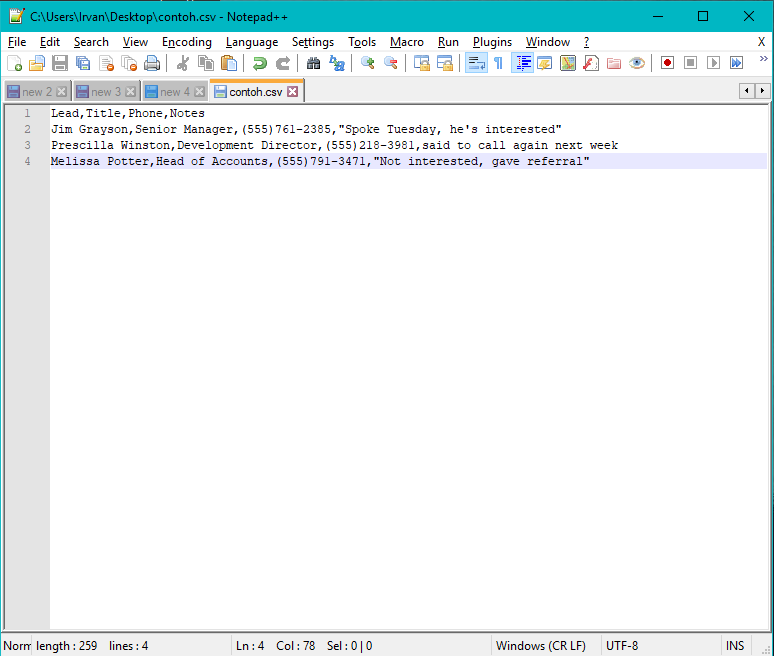
\includegraphics[width=0.6\textwidth]{figures/chapter4/Contoh_CSV.png}}
							\caption{Contoh CSV}
							\label{Contoh CSV}
						\end{figure}

					\ref{Contoh_CSV}
				\end{itemize}
			
			\item Ada banyak aplikasi yang dapat membuat file berformat CSV, diantaranya adalah :
				\begin{itemize}
					\item Notepad
					\item Notepad++
					\item Microsoft Excel
					\item Corel Quatro Pro
					\item Apache Open Office, dan masih banyak yang lainnya.
				\end{itemize}
			
			\item Cara menulis file csv menggunakan Excel :
				\begin{enumerate}
					\item Buka aplikasi Microsoft Excel kemudian buat dokumen baru
					\item Tulis judul kolom untuk setiap informasi yang ingin di rekam atau catat, kemudian tulis informasi - informasi dalam kolom dengan sesuai.
					\item Jika sudah selesai maka save dengan cara pilih menubar File lalu pilih Save As
					\item Lalu isikan nama file tersebut dan rubah dengan memilih format file yang tersedia tersebut menjadi .csv
					\item File csv sudah berhasil terbuat menggunakan Microsoft Excel
				\end{enumerate}
			\item Cara membaca file csv menggunakan Excel :
				\begin{enumerate}
					\item Buka aplikasi Microsoft Excel kemudian pilih menu Open
					\item Cari tempat file csv yang ingin dibuka, kemudian pilih Open
					\item File csv sudah berhasil dibaca menggunakan Microsoft Excel
				\end{enumerate}
			
			\item Pada file csv, tanda baca koma diartikan sebagai pembatas suatu kolom. List-directed input output didefinisikan dalam FORTRAN 77. List-directed input menggunakan tanda baca koma atau spasi sebagi pembatas, sehinnga karakter yang tidak dikutip tidak dapat mengandung tanda baca koma ataupun spasi. Hal tersebut yang diadopsi oleh file csv. format csv didukung dengan library untuk banyak bahasa pemrograman, kebanyakan yang menspesifikasikan pembatas field, pemisah desimal, pengkodean karakter, dan yang lainnya.
			
			\item Pada tahun 2008, pengembangan pandas dimulai oleh AQR Capital Management. Pada akhir tahun 2009 pandas menjadi Open Sourced, dimana disupport oleh banyak komunitas atau individu di dunia untuk mengembangkan pandas. Sejak tahun 2015, pandas menjadi NumFOCUS proyek sponsor, ini juga membantu suksesnya pengembangan dari pandas itu sendiri. pandas merupakan struktur data dan data analysis tools untuk bahasa pemrograman Python, dan merupakan BSD-licensed library yang menjadikannya memiliki performa yang tinggi.
			
			\item 
				\begin {itemize} 
					\item Tanda baca koma : Menjadi pemisah antar kolom
					\item Tanda baca kutip dua : Menjadi cara untuk memasukan sebuah kalimat atau untuk memasukan karakter spasi sebagai data pada kolom informasi
					\item Inputan pada baris pertama akan menjadi Header, dimana akan menjadi nama sebuah kolom, dan masih banyak yang lainnya
				\end{itemize}
			
			\item Pada pandas sedikit berbeda, dimana inputan data berbentuk seperti peng-inputan pada variabel pada umumnya, hanya saja menggunakan tanda kutip satu untuk menandakan sebuah informasi pada kolom kemudian tanda kurung kotak yang didalamnya berisi informasi data dari kolom tersebut. dan lain sebagainya.
			
		\end{enumerate}